% =====================================================================
% Clase -- Trigonometría 10° -- Trimestre I -- Semana 03
% Sesión 009 (mar 15 sep., 11:50, 50 min) · 010 (jue 17 sep., 11:50, 50 min)
% Sesión 011 (jue 17 sep., 13:40, 50 min, taller) · 012 (vie 18 sep., 10:10, 50 min, tarea)
% Tema: Razones trigonométricas
% Hilo conductor del trimestre I: «Medir lo inalcanzable»
% Temas de la guía: 1 (tema:razones) y 5 (tema:rotacion, grados/minutos/segundos)
% Material del docente (no se entrega a los estudiantes).
% =====================================================================
\documentclass[11pt]{article}
\makeatletter\def\input@path{{../../../../../plantillas/estilo/}}\makeatother
\usepackage{mmcantillo}
\guiadelestudiante{../../guia-didactica/guia-periodo-I-medir-lo-inalcanzable}

\tipodocumento{Clase}
\asignatura{Trigonometría}
\titulo{Semana 3: del ángulo medido a la razón}
\grado{10°}
\periodo{I}

% DBA: matematicas grado 10 · DBA 4 — Comprende y utiliza funciones para modelar
% fenómenos periódicos y justifica las soluciones. Evidencia 1: «Reconoce el significado
% de las razones trigonométricas en un triángulo rectángulo para ángulos agudos, en
% particular, seno, coseno y tangente.» Las cuatro sesiones de la semana construyen esa
% evidencia: medir el ángulo (009), ver que la razón solo depende de él (010-011) y
% nombrarla seno, coseno y tangente (012).

\begin{document}

\encabezado*

\begin{center}
{\renewcommand{\arraystretch}{1.3}
\begin{tabularx}{\linewidth}{@{}l l l X l@{}}
  \toprule
  \textbf{Sesión} & \textbf{Fecha} & \textbf{Min} & \textbf{Subtema} & \textbf{Entregables}\\
  \midrule
  009 & mar 15 sep., 11:50 & 50 & Ángulos: sistema sexagesimal (grados, minutos y
      segundos) y clasificación & ---\\
  010 & jue 17 sep., 11:50 & 50 & De la semejanza a la razón: en triángulos rectángulos
      semejantes la razón depende solo del ángulo & ---\\
  011 & jue 17 sep., 13:40 & 50 & Taller: medir lados en triángulos semejantes y comparar
      sus razones & Taller (en clase)\\
  012 & vie 18 sep., 10:10 & 50 & Definición de seno, coseno y tangente (cateto opuesto,
      adyacente, hipotenusa) & Tarea (para el mar 22 sep.)\\
  \bottomrule
\end{tabularx}}
\end{center}

La semana 02 cerró el refuerzo de semejanza y Pitágoras. Esta semana esa semejanza se
convierte en la herramienta del año: si dos triángulos rectángulos tienen el mismo ángulo
agudo, la razón entre dos de sus lados es la misma aunque los triángulos sean de tamaños
muy distintos. Ese es el paso que permite «medir lo inalcanzable».
Referencias: \refguia{tema:razones} y \refguia{tema:rotacion}.

\begin{nota}
\textbf{Orden de la semana.} El nombre de las razones (seno, coseno, tangente) se reserva
para la sesión 012 a propósito. En las sesiones 010 y 011 los estudiantes solo miden y
dividen: la idea de que «la razón depende solo del ángulo» se descubre antes de tener un
nombre para ella. Si alguien ya trae los nombres de otro curso, se aceptan, pero el taller
se responde con medidas.
\end{nota}

% ---------------------------------------------------------------------
\seccion{Sesión 009 — martes 15 de septiembre · 11:50 · 50 min}

\textbf{Objetivo.} Medir y escribir ángulos en el sistema sexagesimal (grados, minutos y
segundos), pasar de grados-minutos-segundos a grados decimales y de vuelta, y clasificar
ángulos por su medida.

\textbf{Materiales.} Tablero; transportador; calculadora científica; la guía del estudiante.

\begin{center}
{\renewcommand{\arraystretch}{1.3}
\begin{tabularx}{\linewidth}{@{}l l X@{}}
  \toprule
  \textbf{Momento} & \textbf{Min} & \textbf{Actividad}\\
  \midrule
  Enganche & 0--6 & Leer el recuadro del hilo: en 1850 Agustín Codazzi sale a levantar el
    mapa de la Nueva Granada. No puede caminar cada montaña; mide ángulos. Pregunta al
    grupo: «¿con qué precisión hay que medir un ángulo para que un mapa sirva?»\\
  Sexagesimal & 6--18 & De dónde viene el 60 (babilonios) y por qué sobrevivió: un grado
    se parte en $60$ minutos ($1^\circ = 60'$) y un minuto en $60$ segundos ($1' = 60''$).
    Escribir en el tablero la conversión en los dos sentidos con el ejemplo de la guía:
    $40^\circ\,30' = \num{40,5}^\circ$. Segundo ejemplo, más fino:
    $7^\circ\,12' = 7^\circ + \frac{12}{60}^{\circ} = \num{7,2}^\circ$ (el ángulo de
    Eratóstenes, que volverá en el tema de radianes).\\
  Al revés & 18--28 & De decimal a sexagesimal: $\num{23,45}^\circ$. La parte entera son
    $23^\circ$; $\num{0,45}\times 60 = 27$, luego $23^\circ\,27'$. Señalar que esa es
    justamente la latitud que aparece en los mapas de Cali ($3^\circ\,27'$ norte). Mostrar
    la tecla \texttt{$^\circ$\,'\,''} de la calculadora y advertir el error típico:
    \emph{$23^\circ\,45'$ no es $\num{23,45}^\circ$}.\\
  Clasificación & 28--38 & Repaso rápido, con el transportador en la mano: agudo
    ($<90^\circ$), recto ($=90^\circ$), obtuso (entre $90^\circ$ y $180^\circ$), llano
    ($=180^\circ$), completo ($=360^\circ$). Complementarios (suman $90^\circ$) y
    suplementarios (suman $180^\circ$): se usarán toda la unidad, porque los dos ángulos
    agudos de un triángulo rectángulo son complementarios.\\
  Práctica & 38--48 & En parejas, en el cuaderno: (1) pasar a decimal $18^\circ\,30'$,
    $52^\circ\,15'$ y $6^\circ\,45'$; (2) pasar a grados y minutos $\num{74,8}^\circ$ y
    $\num{12,25}^\circ$; (3) decir de qué tipo es cada ángulo y cuál es su complemento
    cuando exista. La docente pasa por los puestos.\\
  Cierre & 48--50 & Idea clave: \emph{un ángulo se mide, y medirlo bien es lo que sostiene
    un mapa}. Anunciar la pregunta del jueves: «¿hace falta medir el triángulo grande?»\\
  \bottomrule
\end{tabularx}}
\end{center}

\textbf{Respuestas de la práctica.}
\begin{enumerate}
  \item $18^\circ\,30' = \num{18,5}^\circ$; \quad $52^\circ\,15' = \num{52,25}^\circ$;
    \quad $6^\circ\,45' = \num{6,75}^\circ$.
  \item $\num{74,8}^\circ = 74^\circ\,48'$ (porque $\num{0,8}\times 60 = 48$); \quad
    $\num{12,25}^\circ = 12^\circ\,15'$.
  \item $18^\circ\,30'$, $52^\circ\,15'$, $6^\circ\,45'$ y $\num{74,8}^\circ$ son agudos;
    sus complementos son $71^\circ\,30'$, $37^\circ\,45'$, $83^\circ\,15'$ y
    $15^\circ\,12'$. Un ángulo obtuso o llano no tiene complemento.
\end{enumerate}

\begin{nota}
Si el grupo avanza rápido, adelantar el dato del recuadro «La Tierra gira $15^\circ$ por
hora» de la guía: $360^\circ \div 24 = 15^\circ$, y por eso Colombia (hacia los $75^\circ$
de longitud oeste) va cinco horas detrás de Greenwich. Es un ángulo que se vuelve tiempo.
\end{nota}

% ---------------------------------------------------------------------
\seccion{Sesión 010 — jueves 17 de septiembre · 11:50 · 50 min}

\textbf{Objetivo.} Descubrir que, en triángulos rectángulos semejantes, la razón entre dos
lados depende solo del ángulo agudo y no del tamaño del triángulo.

\textbf{Materiales.} Tablero; regla y transportador; calculadora; la guía del estudiante.

\begin{center}
{\renewcommand{\arraystretch}{1.3}
\begin{tabularx}{\linewidth}{@{}l l X@{}}
  \toprule
  \textbf{Momento} & \textbf{Min} & \textbf{Actividad}\\
  \midrule
  Enganche & 0--7 & El recuadro del hilo del Tema 1: Tales en Egipto clava un palo y
    compara su sombra con la de la pirámide. Los rayos del Sol llegan con la misma
    inclinación, así que los dos triángulos son semejantes. Pregunta: «¿qué medimos
    realmente? ¿la pirámide o el palo?»\\
  Construcción & 7--22 & En el tablero, tres triángulos rectángulos con el mismo ángulo
    $\theta = 35^\circ$ y catetos horizontales $4$, $6$ y $10$ cm. Con el grupo: son
    semejantes (dos ángulos iguales). Llenar la tabla de la figura de abajo con las
    razones $\frac{\text{vertical}}{\text{horizontal}}$ y
    $\frac{\text{vertical}}{\text{hipotenusa}}$. Salen iguales.\\
  ¿Por qué? & 22--32 & La demostración de la guía, en una línea: si los lados del grande
    son $k$ veces los del pequeño, en cada razón se multiplican por $k$ el numerador
    \emph{y} el denominador, y la razón no cambia. Escribirlo:
    $\dfrac{k\,a}{k\,c} = \dfrac{a}{c}$. Conclusión: la razón es una propiedad
    \emph{del ángulo}, no del triángulo.\\
  Nombrar los lados & 32--42 & Con la figura de la guía: hipotenusa (frente al ángulo
    recto), cateto opuesto (frente a $\theta$) y cateto adyacente. Insistir en que
    «opuesto» y «adyacente» cambian si se mira desde el otro ángulo agudo: hacerlo girar
    en el tablero con el mismo triángulo.\\
  Anticipo & 42--50 & Volver a Tales: sombra del palo $=2$ m, palo $=1{,}5$ m, sombra de
    la pirámide $=$ unos $190$ m. Razón $\frac{\text{altura}}{\text{sombra}}
    = \frac{1{,}5}{2} = \num{0,75}$, luego la pirámide mide $190 \times \num{0,75}
    \approx 143$ m. Anunciar el taller de la sesión siguiente.\\
  \bottomrule
\end{tabularx}}
\end{center}

\textbf{Figura para el tablero (los tres triángulos semejantes).}

\begin{center}
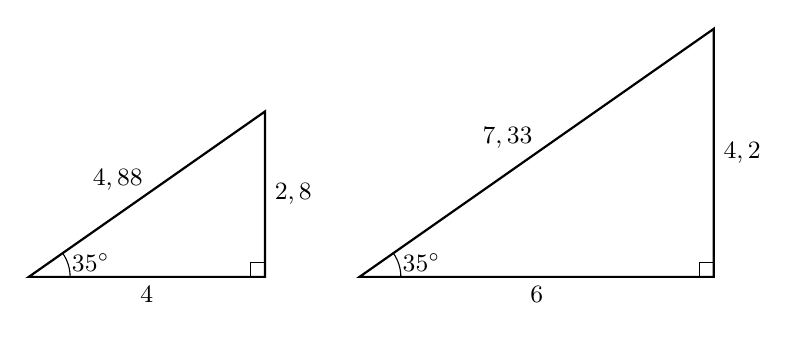
\begin{tikzpicture}[scale=0.75, every node/.style={font=\small}]
  % T1
  \begin{scope}[xshift=0cm]
    \pgfmathsetmacro\h{4*0.7002}
    \draw[thick] (0,0) -- (4,0) -- (4,\h) -- cycle;
    \draw (3.75,0) -- (3.75,0.25) -- (4,0.25);
    \draw (0.7,0) arc (0:35:0.7); \node at (1.05,0.24) {$35^\circ$};
    \node[below] at (2,0) {$4$}; \node[right] at (4,\h/2) {$\num{2,8}$};
    \node[above left=-2pt] at (2,\h/2) {$\num{4,88}$};
  \end{scope}
  % T2
  \begin{scope}[xshift=5.6cm]
    \pgfmathsetmacro\h{6*0.7002}
    \draw[thick] (0,0) -- (6,0) -- (6,\h) -- cycle;
    \draw (5.75,0) -- (5.75,0.25) -- (6,0.25);
    \draw (0.7,0) arc (0:35:0.7); \node at (1.05,0.24) {$35^\circ$};
    \node[below] at (3,0) {$6$}; \node[right] at (6,\h/2) {$\num{4,2}$};
    \node[above left=-2pt] at (3,\h/2) {$\num{7,33}$};
  \end{scope}
\end{tikzpicture}

{\small Con $\theta = 35^\circ$: $\dfrac{\num{2,8}}{4} = \dfrac{\num{4,2}}{6} = \num{0,70}$
\quad y \quad $\dfrac{\num{2,8}}{\num{4,88}} = \dfrac{\num{4,2}}{\num{7,33}} = \num{0,57}$.}
\end{center}

\begin{nota}
El tercer triángulo ($b = 10$, vertical $\num{7,0}$, hipotenusa $\num{12,21}$) se deja para
que lo complete el grupo en el cuaderno: es la comprobación de que el patrón no depende del
dibujo del tablero. Las razones dan $\num{0,70}$ y $\num{0,57}$ otra vez.
\end{nota}

% ---------------------------------------------------------------------
\seccion{Sesión 011 — jueves 17 de septiembre · 13:40 · 50 min (taller)}

\textbf{Objetivo.} Comprobar con regla y transportador, sobre triángulos que los
estudiantes miden, que la razón entre dos lados solo depende del ángulo.

\textbf{Materiales.} El taller impreso (\texttt{taller.tex}); regla graduada en milímetros;
transportador; calculadora.

\begin{center}
{\renewcommand{\arraystretch}{1.3}
\begin{tabularx}{\linewidth}{@{}l l X@{}}
  \toprule
  \textbf{Momento} & \textbf{Min} & \textbf{Actividad}\\
  \midrule
  Instrucciones & 0--6 & Repartir el taller. Recordar que se mide en milímetros y se
    escriben las medidas \emph{antes} de dividir; una diferencia en la segunda cifra
    decimal es normal y no es un error.\\
  Trabajo & 6--38 & Individual, con consulta al compañero. La docente pasa revisando que
    midan la hipotenusa y no el lado vertical, y que dividan en el orden pedido.\\
  Puesta en común & 38--48 & Recoger en el tablero las razones de cuatro o cinco
    estudiantes para el mismo triángulo y compararlas. Deben coincidir en las dos primeras
    cifras. Discutir de dónde viene la diferencia (el grosor del lápiz, la regla, el
    dibujo), no del concepto.\\
  Cierre & 48--50 & Anunciar que el viernes esas razones reciben por fin un nombre.\\
  \bottomrule
\end{tabularx}}
\end{center}

\begin{nota}
El taller se califica sobre \textbf{5 puntos} y se recoge al final de la sesión. Si alguien
termina antes, pedirle que dibuje un cuarto triángulo con el mismo ángulo y otro tamaño y
verifique que la razón se repite.
\end{nota}

% ---------------------------------------------------------------------
\seccion{Sesión 012 — viernes 18 de septiembre · 10:10 · 50 min}

\textbf{Objetivo.} Definir seno, coseno y tangente de un ángulo agudo, usar la calculadora
en modo grados en los dos sentidos y hallar un lado de un triángulo rectángulo.

\textbf{Materiales.} Tablero; calculadora científica (una por pareja como mínimo); la guía;
la tarea impresa.

\begin{center}
{\renewcommand{\arraystretch}{1.3}
\begin{tabularx}{\linewidth}{@{}l l X@{}}
  \toprule
  \textbf{Momento} & \textbf{Min} & \textbf{Actividad}\\
  \midrule
  Recoger el hilo & 0--6 & Volver a los números del taller: todos obtuvieron
    aproximadamente lo mismo. Esas razones ya tienen nombre desde hace más de mil años.\\
  Definición & 6--18 & Escribir la definición del Tema 1 de la guía:
    $\sen\theta = \frac{\text{op}}{\text{hip}}$,
    $\cos\theta = \frac{\text{ady}}{\text{hip}}$,
    $\tg\theta = \frac{\text{op}}{\text{ady}}$. Volver a la tabla de la sesión 010: lo que
    llamaban $\frac{\text{vertical}}{\text{horizontal}}$ era $\tg 35^\circ$, y
    $\frac{\text{vertical}}{\text{hipotenusa}}$ era $\sen 35^\circ$. Comprobar con la
    calculadora: $\tg 35^\circ \approx \num{0,7002}$ y $\sen 35^\circ \approx \num{0,5736}$.\\
  Calculadora & 18--30 & Modo DEG (y qué pasa en RAD: $\sen 30$ da $\num{-0,988}$ en vez de
    $\num{0,5}$ — señal de alarma). Las teclas $\texttt{sin}^{-1}$, $\texttt{cos}^{-1}$,
    $\texttt{tan}^{-1}$ hacen el camino de vuelta: de la razón al ángulo. Ejemplos del
    Tema 1: $\sen\theta = \num{0,2164} \Rightarrow \theta \approx \num{12,5}^\circ$.\\
  Hallar un lado & 30--42 & El ejemplo de la guía: hipotenusa $35$, ángulo $29^\circ$,
    cateto opuesto $x$. Se elige la razón que contiene \emph{lo que sé y lo que busco}:
    $\sen 29^\circ = \frac{x}{35}$, luego $x = 35\sen 29^\circ \approx \num{17,0}$. Hacer
    en el tablero uno con coseno: cateto adyacente $24$, ángulo $40^\circ$, hipotenusa
    $x = \frac{24}{\cos 40^\circ} \approx \num{31,3}$.\\
  Práctica guiada & 42--48 & Preguntas 1 y 2 del Tema 1 de la guía, en parejas, con
    calculadora.\\
  Cierre y tarea & 48--50 & Asignar la tarea, para el martes 22 de septiembre.\\
  \bottomrule
\end{tabularx}}
\end{center}

\textbf{Respuestas de la práctica guiada} (preguntas del Tema 1 de la guía).
\begin{enumerate}
  % Ejercicio: razones-trigonometricas-10-001, razones-trigonometricas-10-003, razones-trigonometricas-10-005
  \item $\sen\num{41,3}^\circ \approx \num{0,6600}$; \quad
    $\tg\num{54,4}^\circ \approx \num{1,3968}$; \quad
    $\cos\num{49,2}^\circ \approx \num{0,6534}$.
  % Ejercicio: razones-trigonometricas-10-007, razones-trigonometricas-10-009
  \item $\sen\theta = \num{0,2164} \Rightarrow \theta \approx \num{12,5}^\circ$; \quad
    $\tg\theta = \num{0,3096} \Rightarrow \theta \approx \num{17,2}^\circ$.
\end{enumerate}

\begin{nota}
\textbf{Error típico.} Elegir la razón por costumbre y no por los datos. Conviene dejar en
el tablero, durante toda la unidad, la pregunta de tres pasos: ¿qué lado conozco?, ¿qué
lado busco?, ¿qué razón los contiene a los dos? La calculadora no lo decide.
\end{nota}

\end{document}
